%% LyX 2.0.6 created this file.  For more info, see http://www.lyx.org/.
%% Do not edit unless you really know what you are doing.
\documentclass[english]{article}
\usepackage[T1]{fontenc}
\usepackage[latin9]{inputenc}
\usepackage{graphicx}
\usepackage{babel}
\begin{document}

\title{Homework 6}


\author{Alexander Gould}

\maketitle
3A. $A\cup B=\left\{ 0,1,2,3,4,5,6\right\} $

3B. $A\cap B=\left\{ 3\right\} $

3C. $A-B=\left\{ 1,2,4,5\right\} $

3D. $B-A=\left\{ 0,6\right\} $

14. $A=\left\{ 1,3,5,6,7,8,9\right\} $, $B=\left\{ 2,3,6,9,10\right\} $

15A. Any $x\in\overline{A\cap B}$ is obviously $\notin A\cap B$,
meaning $x\notin A\vee x\notin B$, or $x\in\overline{A}\vee x\in\overline{B}$.
This means that $x\in\overline{A}\cup\overline{B}$, which shows that
$\overline{A\cap B}\subseteq\overline{A}\cup\overline{B}$. Any $x\in\overline{A}\cup\overline{B}$
is obviously $x\in\overline{A}\vee x\in\overline{B}$, meaning $x\notin A\vee x\notin B$,
or $x\in\overline{A}\vee x\in\overline{B}$$\notin A\cap B$. This
means that $x\in\overline{A\cap B}$, which shows that $\overline{A\cap B}\subseteq\overline{A}\cup\overline{B}$.

18E. $x\in\left(B-A\right)\cup\left(C-A\right)$ translates to $x\in\left(B-A\right)\vee x\in\left(C-A\right)$.
We can further expand this to $\left(x\in B\wedge x\notin A\right)\vee\left(x\in C\wedge x\notin A\right)$.
We can then move the A outside and get $\left(x\in B\vee x\in C\right)\wedge x\notin A$.
This becomes $x\in B\cup C\wedge x\notin A$. We can use the definition
of set subtration to get to $x\in\left(B\cup C\right)-A$.

19A. $x\in\left(A-B\right)$ can become $x\in A\wedge x\notin B$.
We can rewrite this in set notation as $x\in A\cap\overline{B}$.
Going the other way, $x\in A\cap\overline{B}$ becomes $x\in A\wedge x\notin B$,
which becomes $x\in\left(A-B\right)$.

19B. First we rewrite $x\in\left(A\cap B\right)\cup\left(A\cap\overline{B}\right)$
as $\left(x\in A\wedge x\in B\right)\vee\left(x\in A\wedge x\notin B\right)$.
We can ``factor out'' the $x\in A$, leaving us with $x\in A\wedge\left(x\in B\vee x\notin B\right)$.
The second condition will always be true, and since it's one of 2
parts of an AND, we can just eliminate it and evaluate the other statement,
leaving $x\in A$.

26A.

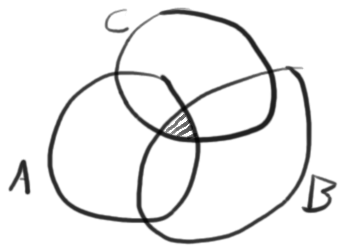
\includegraphics{venn/26A}

26B.

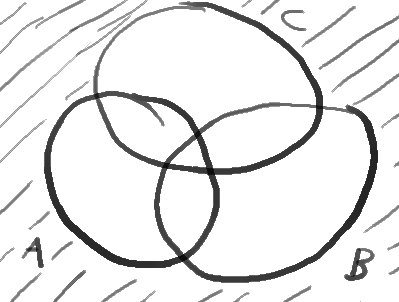
\includegraphics{venn/26B}

26C.

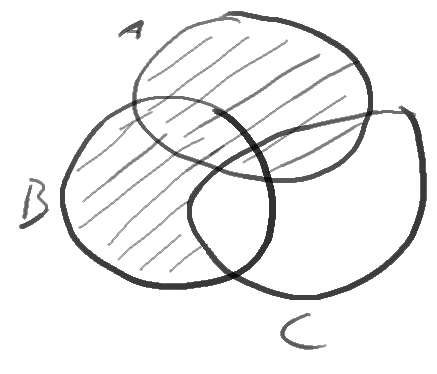
\includegraphics{venn/26C}

29A. If A is equivelant to the union of A and B, we know that B is
empty.

29B. If the intersection of A and B is A, we know A is a subset of
B.

29C. If A-B is A, we know A and B don't intersect.

29D. Knowing that the intersection of A and B and the intersection
of B and A are the same doesn't tell us anything. Intersection is
commutative.

29E. When $A-B=B-A$, we know that sets are equal.

32. $\left\{ 2,5\right\} $

35. $x\in A\bigoplus B$ means that $\left(x\in A\vee x\in B\right)\wedge\left(x\notin A\vee x\notin B\right)$.
Use DeMorgan's law to simplify this to $\left(x\in A\vee x\in B\right)\wedge\neg\left(x\in A\wedge x\in B\right)$.
Rewrite this as $x\in A\cup B\wedge\neg\left(x\in A\cap B\right)$,
and use the definition of set subtraction to get $x\in\left(A\cup B\right)-\left(A\cap B\right)$

41. Yes. In order for 2 set pairs to have the same symmetric difference,
both their unions and intersections must be identical. That can only
happen if you're comparing the same 2 sets.

50A. The union would contain every number from 1 to $\infty$. The
intersection would be empty.

50B. The union would contain every number from 0 to $\infty$. The
intersection would contain 0.

50C. The union would contain every number from 0 to $\infty$. The
intersection would contain 1.

50D. The union would contain every number from 1 to $\infty$. The
intersection would be empty/contain only $\infty$.
\end{document}
